\section{Tries}
\subsection{Regular Tries}
A trie is a tree-based data structure for storing strings where each path from
the root represents a sequence of characters. Words sharing common prefixes
share the same path through the tree, making tries space-efficient for storing
related strings like dictionaries. Each node can be marked to indicate the end
of a valid word, allowing the structure to distinguish between prefixes and
complete words. Operations like insertion, deletion, and lookup run in
$\BigO(m)$ time where m is the length of the string, independent of how many
words are stored. This makes tries particularly useful for tasks like
autocomplete, spell checking, and IP routing where prefix matching is
essential.

\begin{center}
    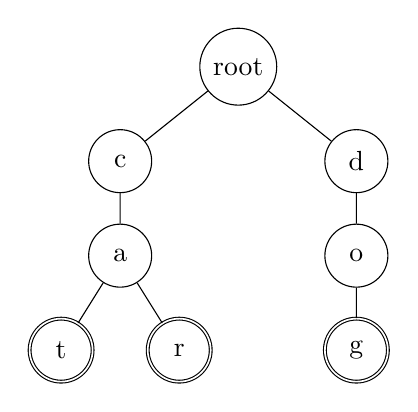
\begin{tikzpicture}[
      level distance=1.2cm,
      level 1/.style={sibling distance=3cm},
      level 2/.style={sibling distance=1.5cm},
      every node/.style={circle, draw, minimum size=0.8cm}
    ]

    \node {root}
      child {node {c}
        child {node {a}
          child {node[double] {t}}
          child {node[double] {r}}
        }
      }
      child {node {d}
        child {node {o}
          child {node[double] {g}}
        }
      };

    \end{tikzpicture}
\end{center}

\subsection{Compact Tries}
A compact trie improves upon the standard trie by compressing chains of nodes
with single children into single edges labeled with strings rather than
individual characters. This significantly reduces space usage from $\BigO(n)$
to $\BigO(s)$ where $s$ is the number of strings stored, making it more
practical for large datasets. The time complexity remains the same as standard
tries since we can still traverse character-by-character along compressed
edges.

\begin{center}
    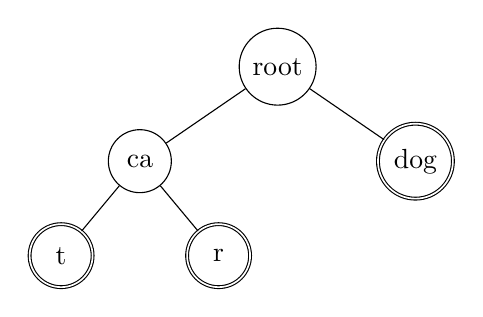
\begin{tikzpicture}[
      level distance=1.2cm,
      level 1/.style={sibling distance=3.5cm},
      level 2/.style={sibling distance=2cm},
      every node/.style={circle, draw, minimum size=0.8cm}
    ]

    \node {root}
      child {node {ca}
        child {node[double] {t}}
        child {node[double] {r}}
      }
      child {node[double] {dog}};

    \end{tikzpicture}
\end{center}

\subsection{Tries Running Time}

\begin{table}[H]
    \centering
    \begin{tabular}{c|c|c|c|c|c}
        & Search & Prefix Search & Preprocessing Time & Space & Explanation \\
        \hline 
        Trie & $\BigO(m)$ & $\BigO(m+\text{occ})$ & $\BigO(n)$ & $\BigO(n)$ & 
        \makecell{Standard trie stores \\ each character in \\ separate nodes} \\
        \hline
        Compact Trie & $\BigO(m)$ & $\BigO(m+\text{occ})$ & $\BigO(n)$ & $\BigO(s)$ & 
        \makecell{Compresses chains \\ Space: $s$ = \#strings \\ instead of $n$ = total length}
    \end{tabular}
\end{table}
